\chapter{Result analysis and discussion}

Introductory lines...



\section{Experimental setup}
\begin{definition}\label{abc}
Add table prepared here
\end{definition}

\section{Training Performance analysis}

\subsection{Training over view for Mobilnet V2}

\begin{figure}[h]
    \centering
    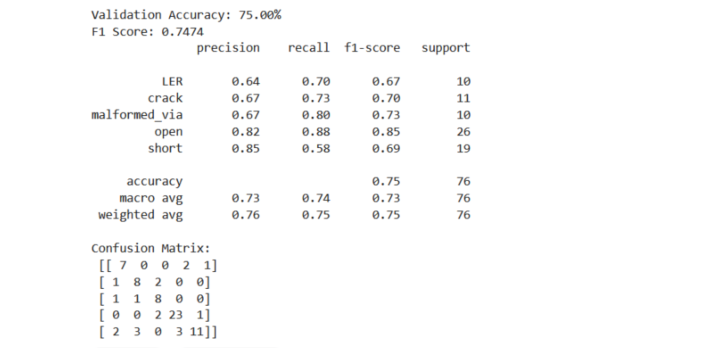
\includegraphics[width=0.8\textwidth]{Images_And_Tables/MobilNetV2_Training.png}
    \caption{MobilnetV2 Training Overview}
    \label{fig:MobilnetV2_Training_Overview}
\end{figure}

\subsubsection{Observation}
The observed accuracy of ~75 \% is expected because MobileNetV2 is a lightweight model optimized for edge deployment. Additionally, INT8 quantization introduces some loss in precision. Given the complexity of SEM images and resource constraints of Raspberry Pi, this represents a reasonable trade-off between accuracy and real-time performance

\subsection{Training over view for Shufflenet}

\begin{figure}[H]
    \centering
    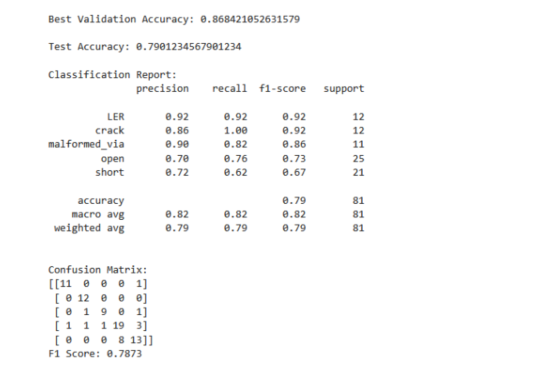
\includegraphics[width=0.8\textwidth]{Images_And_Tables/ShuffleNet_Training.png}
    \caption{ShuffleNet Training Overview}
    \label{fig:ShuffleNet_Training_Overview}
\end{figure}
\subsubsection{Observation}
The ShuffleNet model achieves around 76\% accuracy with an F1-score of 0.75. This is expected given its lightweight architecture, which prioritizes computational efficiency using grouped and depthwise convolutions. The confusion matrix indicates that some defect classes are misclassified due to visual similarity and limited feature representation. However, the model offers significant advantages in terms of low latency and small model size, making it highly suitable for deployment on resource-constrained edge devices like Raspberry Pi


\subsection{Training over view for Resnet18}
\begin{figure}[H]
    \centering
    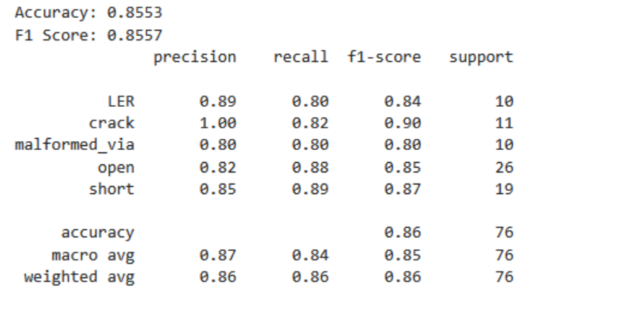
\includegraphics[width=0.8\textwidth]{Images_And_Tables/ResNet18.png}
    \caption{ResNet18 Training Overview}
    \label{fig:ResNet18_Training_Overview}
\end{figure}

\subsubsection{Observation}
ResNet18 achieves the highest accuracy (~85.5\%) due to its deeper architecture and residual learning. However, it is computationally heavy and not suitable for real-time edge deployment, so it is used as a benchmark, while lightweight models are preferred for deployment.

\section{Edge inference result over Raspberry Pi4}

\subsection{Edge inference result for MobilNetV2}
\begin{figure}[H]
    \centering
    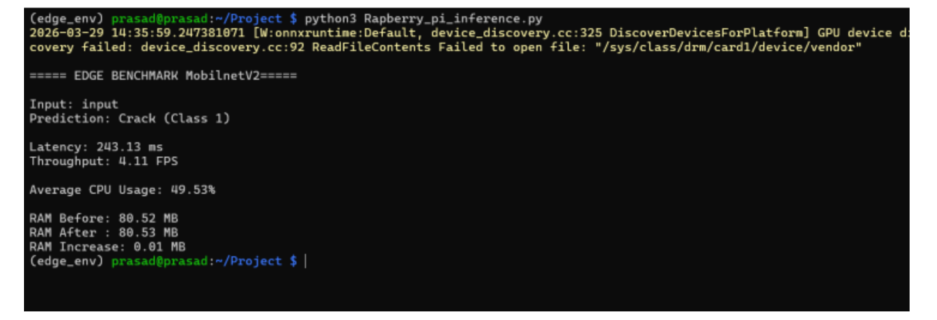
\includegraphics[width=0.8\textwidth]{Images_And_Tables/MobilNetV2_Edge_Inference.png}
    \caption{Edge inference result for MobilNetV2}
    \label{fig:MobilNetV2_Edge_Inference}
\end{figure}


\subsection{Edge inference result for ShuffleNet}
\begin{figure}[H]
    \centering
    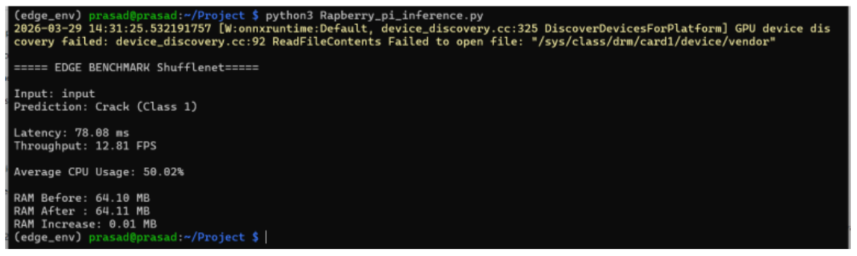
\includegraphics[width=0.8\textwidth]{Images_And_Tables/ShuffleNet_Edge_Inference.png}
    \caption{Edge inference result for ShuffleNet}
    \label{fig:ShuffleNet_Edge_Inference}
\end{figure}

\subsection{Edge inference result for ResNet18}
\begin{figure}[H]
    \centering
    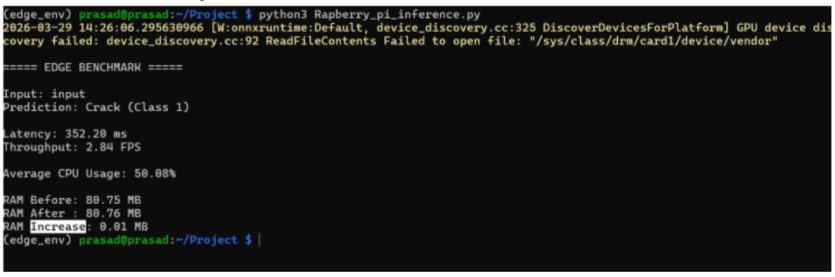
\includegraphics[width=0.8\textwidth]{Images_And_Tables/ResNet18_Edge_Inference.png}
    \caption{Edge inference result for ResNet18}
    \label{fig:ResNet18_Edge_Inference}
\end{figure}

\subsection {Quantitative Model Comparison}

Add Edge Deployment Results \& Comparison table


% Table 1 : Classification Performance
\begin{table}[htbp]
\centering

\footnotesize
\renewcommand{\arraystretch}{1.3}
\setlength{\tabcolsep}{5pt}

\begin{tabular}{|c|c|c|c|c|c|}
\hline
\multicolumn{6}{|c|}{\textbf{Classification Performance}} \\
\hline

\rowcolor{yellow}
\textbf{Sl.No} &
\textbf{Model} &
\textbf{Overall Accuracy} &
\textbf{F1 Score} &
\makecell{\textbf{Model Size in MB} \\ \textbf{After Quantization}} &
\makecell{\textbf{Latency in ms} \\ \textbf{(Kaggle)}} \\
\hline

1 & MobileNetV2 & 0.7530 & 0.7400 & 2.23 & 99.53 \\
\hline
2 & ShuffleNet  & 0.7600 & 0.7594 & 1.30 & 28.19 \\
\hline
3 & ResNet18    & 0.8024 & 0.8552 & 10.70 & 128.71 \\
\hline

\end{tabular}
\caption{Classification Performance of Selected Models}
\label{tab:classification_performance}
\end{table}

% Table 2 : Edge Inference Performance
\begin{table}[htbp]
\centering

\scriptsize
\renewcommand{\arraystretch}{1.3}
\setlength{\tabcolsep}{5pt}

\begin{tabular}{|c|c|c|c|c|c|c|}
\hline
\multicolumn{7}{|c|}{\textbf{Edge Inference Performance}} \\
\hline

\rowcolor{yellow}
\textbf{Sl.No} &
\textbf{Model} &
\textbf{Edge Suitability} &
\textbf{Edge Latency (ms)} &
\textbf{Throughput} &
\makecell{\textbf{Average CPU} \\ \textbf{Usage}} &
\textbf{RAM Increase} \\
\hline

1 & MobileNetV2 & Good      & 244.98 & 4.08  & 49.44 & 0.01 \\
\hline
2 & ShuffleNet  & Excellent & 78.08  & 12.81 & 50.02 & 0.01 \\
\hline
3 & ResNet18    & Poor      & 352.20 & 2.84  & 50.08 & 0.01 \\
\hline

\end{tabular}
\caption{Edge Inference Performance of Selected Models}
\label{tab:edge_inference_performance}
\end{table}

\section{Grad-CAM Qualitative and quantitative analysis}
The model concentrated strongly on the fracture region, indicating that prediction was based on relevant structural discontinuity.

Keep the table for IOU and activation ratio


\begin{table}[htbp]
\centering

\renewcommand{\arraystretch}{1.3}

\begin{tabular}{|c|c|c|c|}
\hline
\rowcolor{yellow}
\textbf{SL. No} & \textbf{Model Used} & \textbf{Mean IOU} & \textbf{Activation Ratio} \\

\hline
1 & ShuffleNet   & 0.2800 & 0.8140 \\
\hline
2 & MobileNetV2  & 0.3135 & 0.8153 \\
\hline
3 & ResNet18     & 0.3576 & 0.8230 \\
\hline

\end{tabular}
\caption{Quantitative Grad-CAM Comparison of Selected Models}
\label{tab:gradcam_comparison}
\end{table}

\subsection{Grad-CAM visualization for MobilenetV2}
\begin{figure}[H]
    \centering
    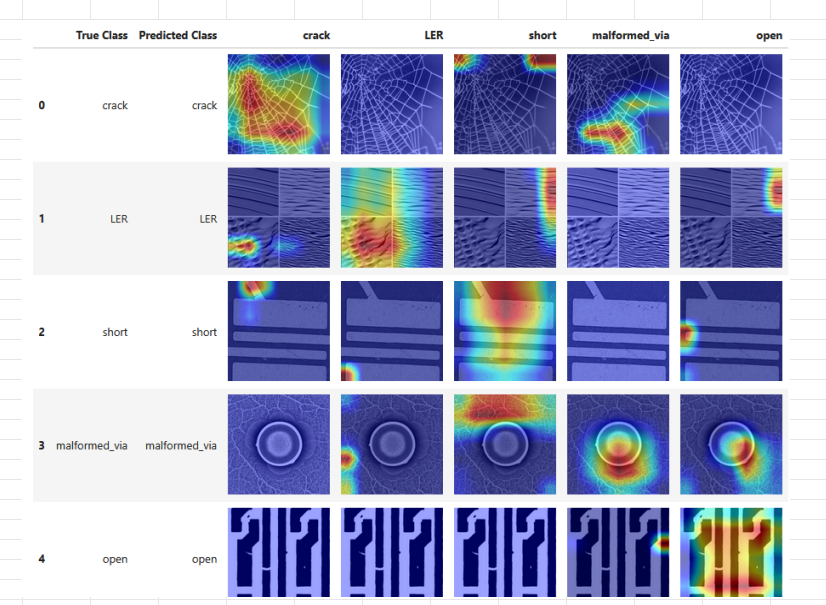
\includegraphics[width=0.6\textwidth]{Images_And_Tables/MobilNet_V2_Grad-Cam.png}
    \caption{Grad-Cam over MobilNetV2}
    \label{fig:Grad-Cam over MobilNetV2}
\end{figure}

\subsection{Grad-CAM visualization for ShuffleNet}
\begin{figure}[H]
    \centering
    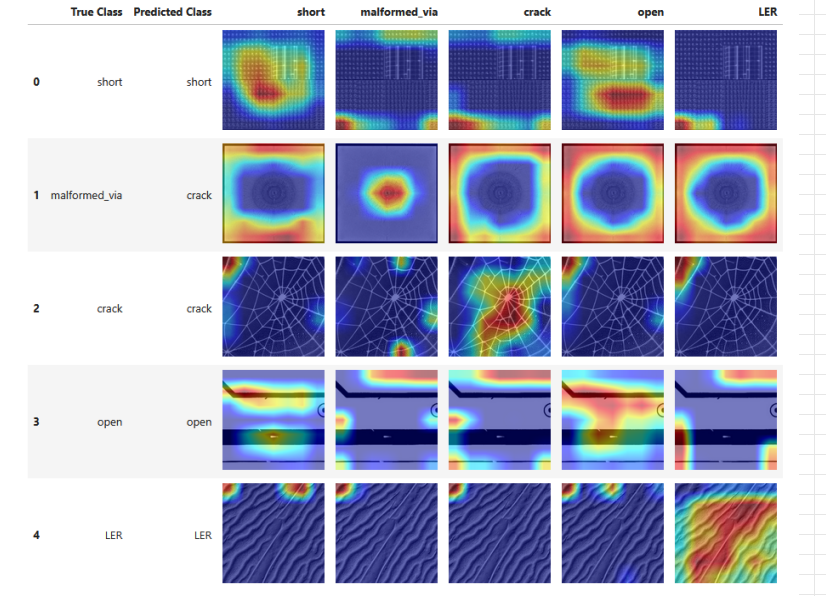
\includegraphics[width=0.6\textwidth]{Images_And_Tables/ShuffleNet_Grad-cam.png}
    \caption{Grad-Cam over ShuffleNet }
    \label{fig:Grad-Cam over ShuffleNet}
\end{figure}

\subsection{Grad-CAM visualization for ResNet18}
\begin{figure}[H]
    \centering
    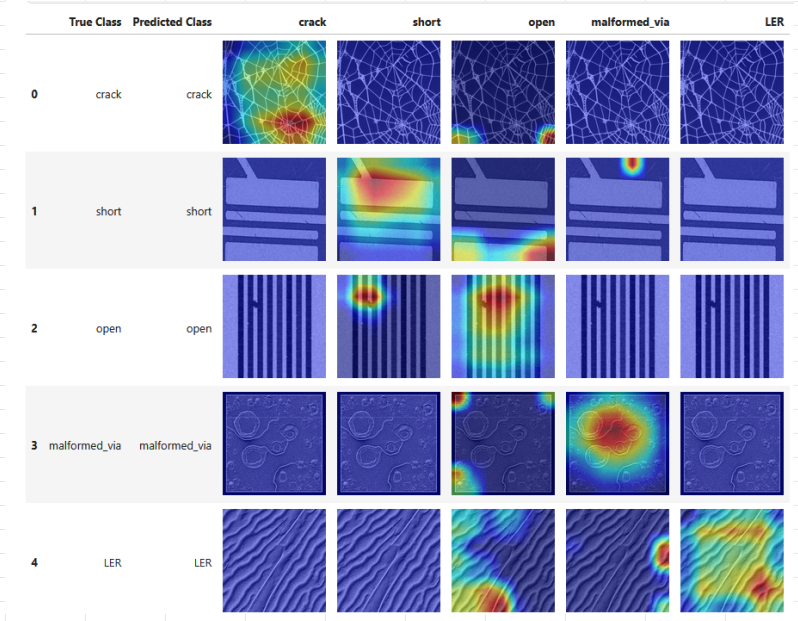
\includegraphics[width=0.6\textwidth]{Images_And_Tables/ReseNet18_Grad-Cam.png}
    \caption{Grad-Cam over ResNet18 }
    \label{fig:Grad-Cam over ResNet18}
\end{figure}
Observations \& Reasoning:
    \begin{itemize}
    \item ResNet18 achieves the highest Mean IoU and activation ratio, indicating better localization of defect regions. This is likely due to its deeper architecture and the presence of residual connections, which help preserve spatial and semantic information across layers, leading to more accurate Grad-CAM heatmaps.
    \item MobileNetV2 performs moderately well. Its inverted residual structure and depthwise separable convolutions make it efficient, but some spatial detail may be lost due to aggressive compression, slightly affecting localization accuracy.
    \item ShuffleNet shows comparatively lower performance. While it is highly optimized for lightweight deployment, the use of channel shuffling and reduced representational capacity may limit its ability to capture fine-grained features required for precise defect localization.
    \end{itemize}

\section{Discussion \& findings}